\section*{Analysis}
\label{Analyse}
%
Based on the results presented in the previous section it is possible to analyse how well a fit the BTL-model and the Preference Tree are.\blankline
%
The total number of possible stochastic violations in the data is 20, where one MST and five SST violations was found. This amount of violations could most likely be described as \textit{some SST violations and few MST violations} and therefore the expectation, as explained in \fullref{Method}, will be that the Preference Tree might fit, but the BTL-model will not. 

To test if the BTL-model could fit a \textit{Chi-square}-test was conducted. The result from the test is a p-value at 0.0055, which is under the significants level at 0.1, and therefore the conclusion is that the BTL-model is significant worse at predicting the data than the statistic model and therefore the model is not accepted as a fit. Instead a Preference Tree was made.\blankline
%
Different types of Preference Trees were tested, but only two Preference Trees was found to have a p-value above 0.1 in the \textit{Chi-square}-tests and therefore not significant different from the statistic model. The two Preference Trees that are concluded to be a fit are illustrated in \fullref{Results} on \autoref{fig:Tree1overveiw} and \autoref{fig:Tree2overveiw} respectively. The value for every line segment of the Preference Tree is calculated. The length of the line segments are presented in \autoref{tab:Length1} for the first Preference Tree and in \autoref{tab:Length2} for the second Preference Tree.  
%
\begin{table}[H]
	\centering
	\begin{tabular}{@{}ll@{}}
		\toprule
		Number of line segment  & Length of line segment \\ \midrule
		1					    & 0.1976   \\
		2      				    & 0.0277   \\
		3      				    & 0.0376   \\
		4      					& 0.0259   \\
		5      					& 0.6931   \\
		6      					& 0.0509   \\
		7      					& 0.8717   \\
		8						& 0.0727   \\ \bottomrule
	\end{tabular}
	\caption{The length of the line segments for the first Preference Tree.}
	\label{tab:Length1}
\end{table} 
\noindent 
% 
\begin{table}[H]
	\centering
	\begin{tabular}{@{}ll@{}}
		\toprule
		Number of line segment  & Length of line segment \\ \midrule
		1						& $3.36\cdot10^{15}$   \\
		2      					& $4.37\cdot10^{14}$   \\
		3      					& $5.98\cdot10^{14}$   \\
		4      					& $7.66\cdot10^{14}$   \\
		5      					& $3.58\cdot10^{16}$   \\
		6     					& $4.00\cdot10^{15}$   \\
		7      					& $1.39\cdot10^{15}$   \\
		8						& $9.69\cdot10^{15}$   \\
		9						& $1.30\cdot10^{15}$   \\ \bottomrule
	\end{tabular}
	\caption{The length of the line segments for the second Preference Tree.}
	\label{tab:Length2}
\end{table} 
\noindent 
%
The scale values for every drug type are calculated by adding all length together for the line segments that leads to the drug. The values are presented in \autoref{tab:ScaleValues1} for the first Preference Tree and in \autoref{tab:ScaleValues2} for the second Preference Tree.\blankline
% 
\begin{table}[H]
	\centering
	\begin{tabular}{@{}ll@{}}
		\toprule
		Drug      & Scale value \\ \midrule
		Alcohol	  & 0.1976   \\
		Tobacco	  & 0.1004   \\
		Cannabis  & 0.1103   \\
		Ecstasy	  & 0.9703   \\
		Heroin	  & 1.6376   \\
		Cocaine	  & 0.9953   \\	\bottomrule
	\end{tabular}
	\caption{The scale values of the different drugs for the first Preference Tree.}
	\label{tab:ScaleValues1}
\end{table} 
\noindent 
%
\begin{table}[H]
	\centering
	\begin{tabular}{@{}ll@{}}
		\toprule
		Drugs     & Scale value \\ \midrule
		Alcohol	  & $3.36\cdot10^{15}$   \\
		Tobacco	  & $1.74\cdot10^{15}$   \\
		Cannabis  & $1.90\cdot10^{15}$   \\
		Ecstasy	  & $1.31\cdot10^{16}$   \\
		Heroin	  & $4.82\cdot10^{16}$   \\
		Cocaine	  & $1.50\cdot10^{16}$   \\	\bottomrule
	\end{tabular}
	\caption{The scale values for the different drugs for the second Preference Tree.}
	\label{tab:ScaleValues2}
\end{table} 
\noindent 
%
To illustrate how the different drugs are rated, the line segments are drawn and labelled, where the labels are found by looking at the types of drugs and considering what is an appropriate description for these specific drugs. On \autoref{fig:Tree1real} the first Preference Tree is illustrated with labels and on \autoref{fig:Tree2real} the second Preference Tree is illustrated. The interpretation of the figures are that the longer the line the higher health risk the drug is rated to have.  
%
\begin{figure}[H]
\centering
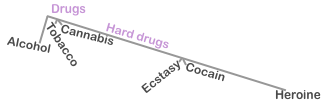
\includegraphics[width = 0.80\textwidth]{Figure/Tree1real}
\caption{The first Preference Tree with correct line length and labels on the line segments.}
\label{fig:Tree1real}
\end{figure}
\noindent
%
\begin{figure}[H]
	\centering
	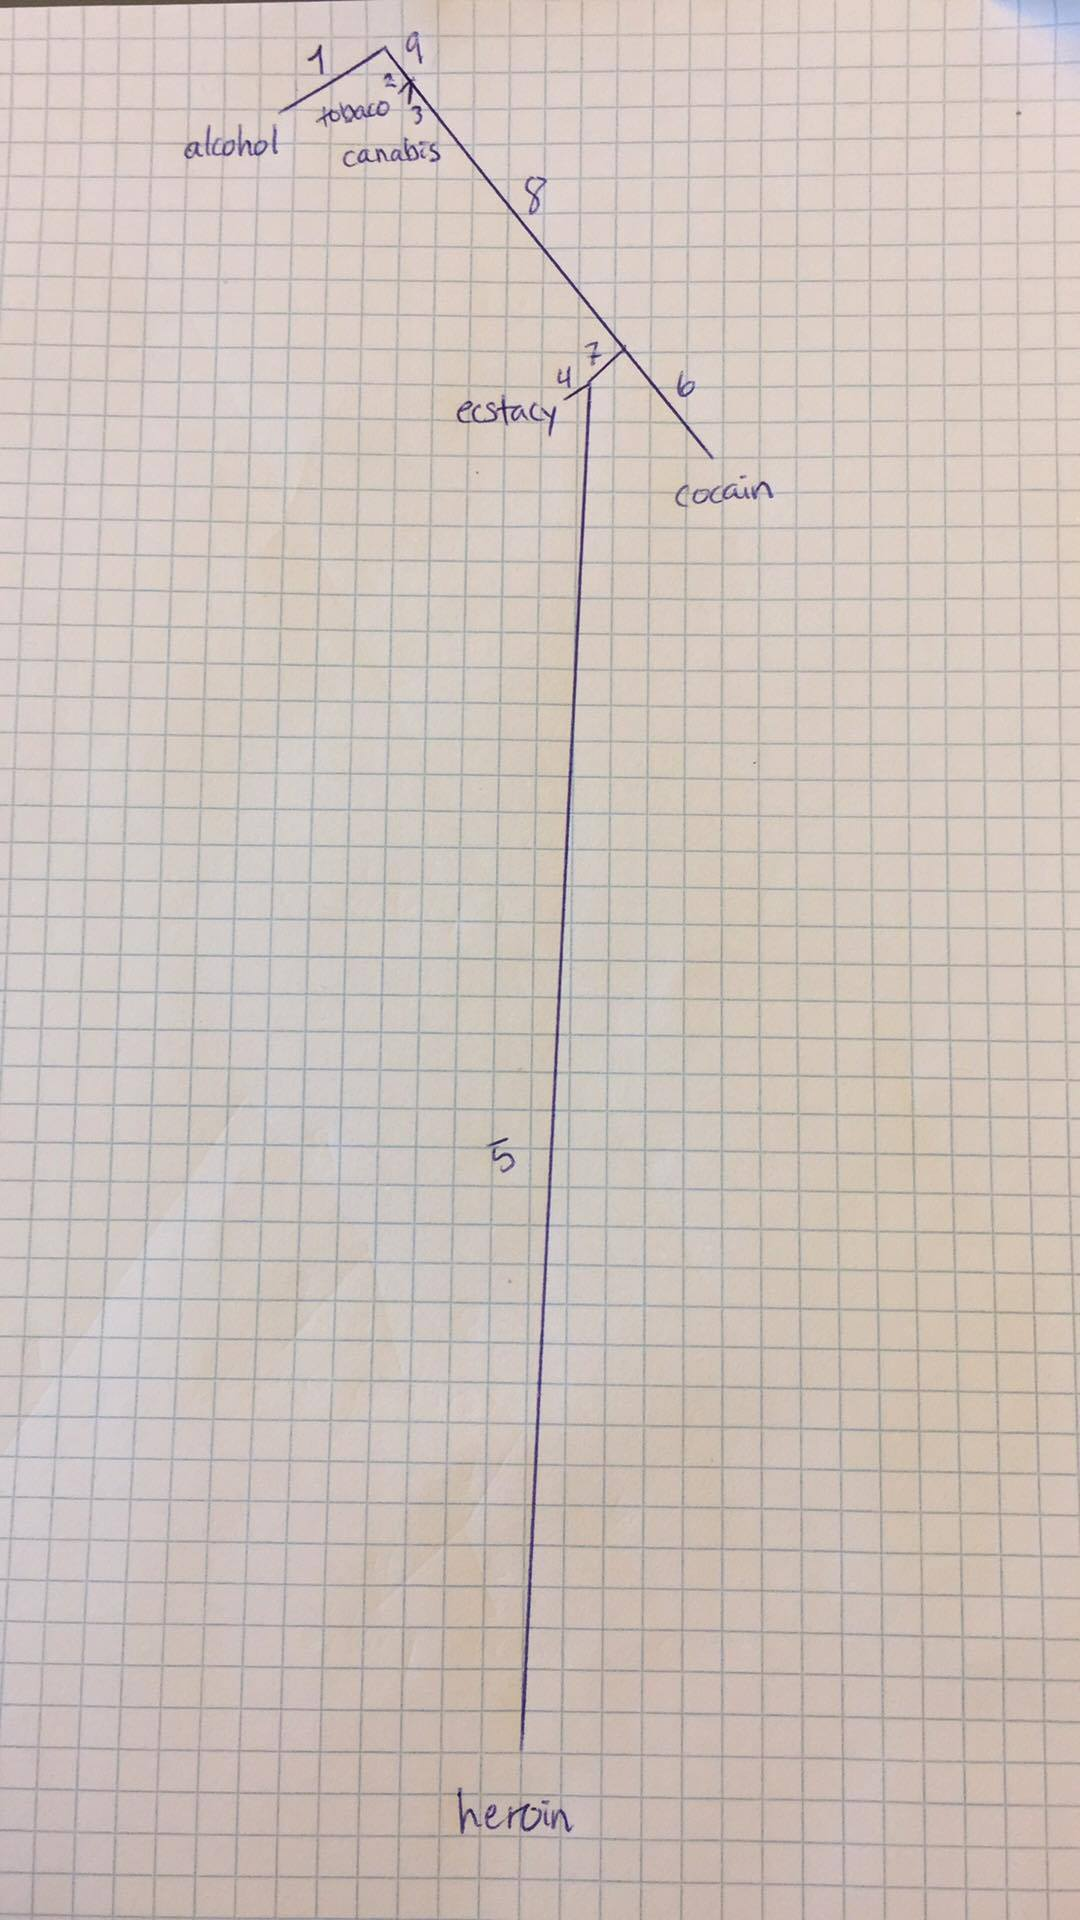
\includegraphics[width = 0.95\textwidth]{Figure/Tree2real}
	\caption{The second Preference Tree with correct line length and labels on the line segments.}
	\label{fig:Tree2real}
\end{figure}
\newpage
\noindent
%
The scale values for the line segments and their respective confidence interval for the first Preference Tree are represented in \autoref{fig:Tree1conf}.
%
\begin{figure}[H]
	\centering
	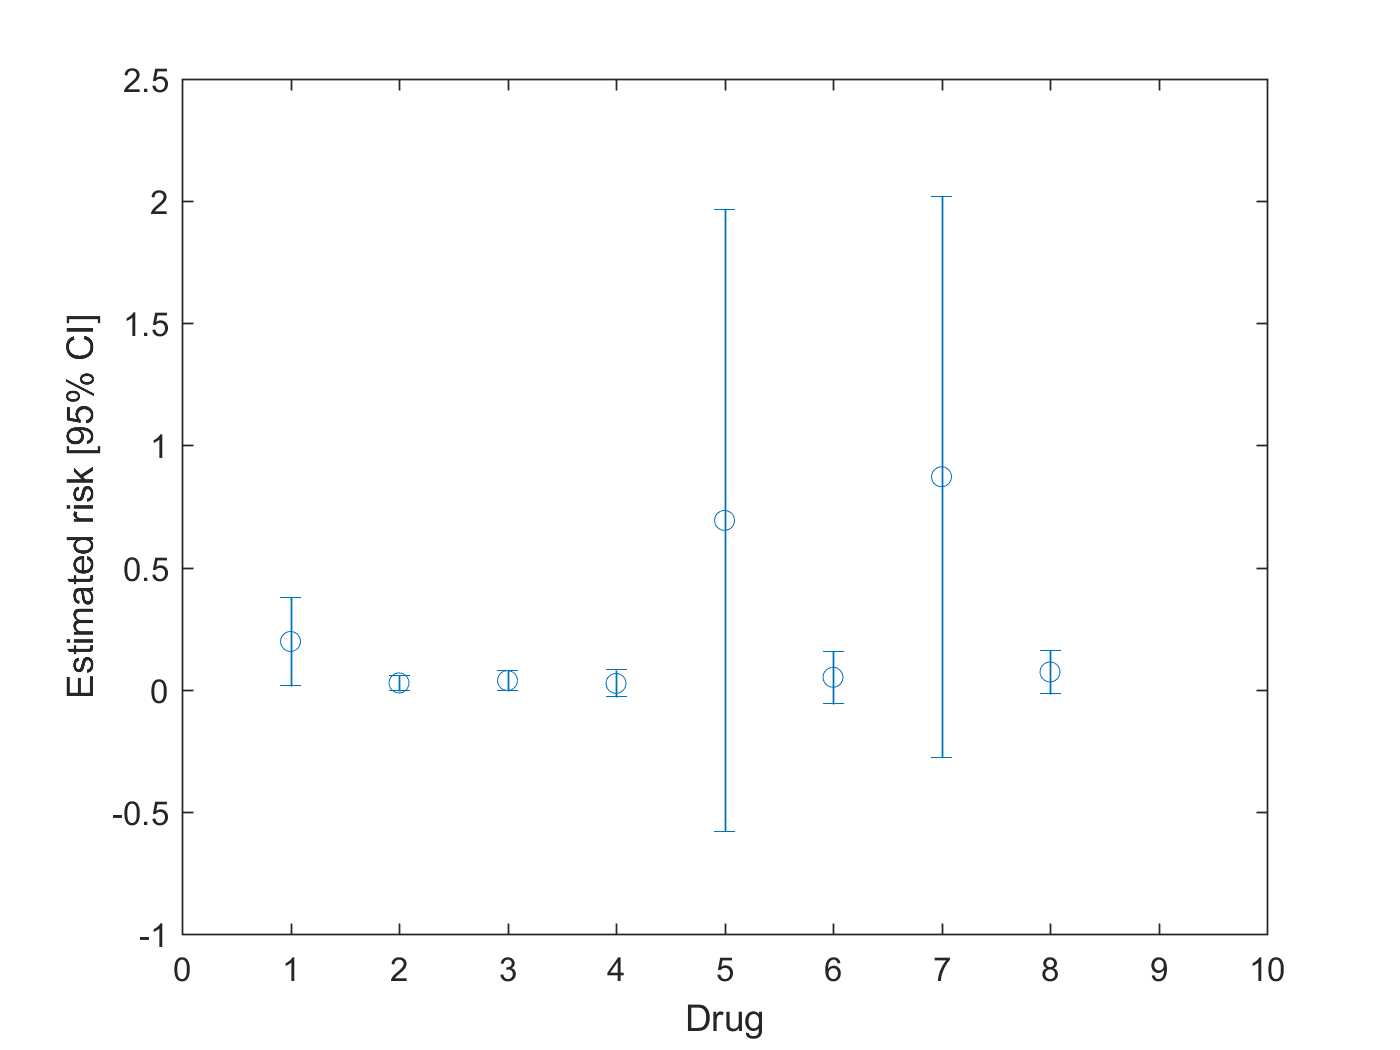
\includegraphics[width = 0.80\textwidth]{Figure/confidense_p1220}
	\caption{Scale values and confidence intervals for the line segments for the first Preference Tree.}
	\label{fig:Tree1conf}
\end{figure}
\noindent
%
The scale values for the line segments and their respective confidence interval for the second Preference Tree are represented in \autoref{fig:Tree2conf}.
%
\begin{figure}[H]
	\centering
	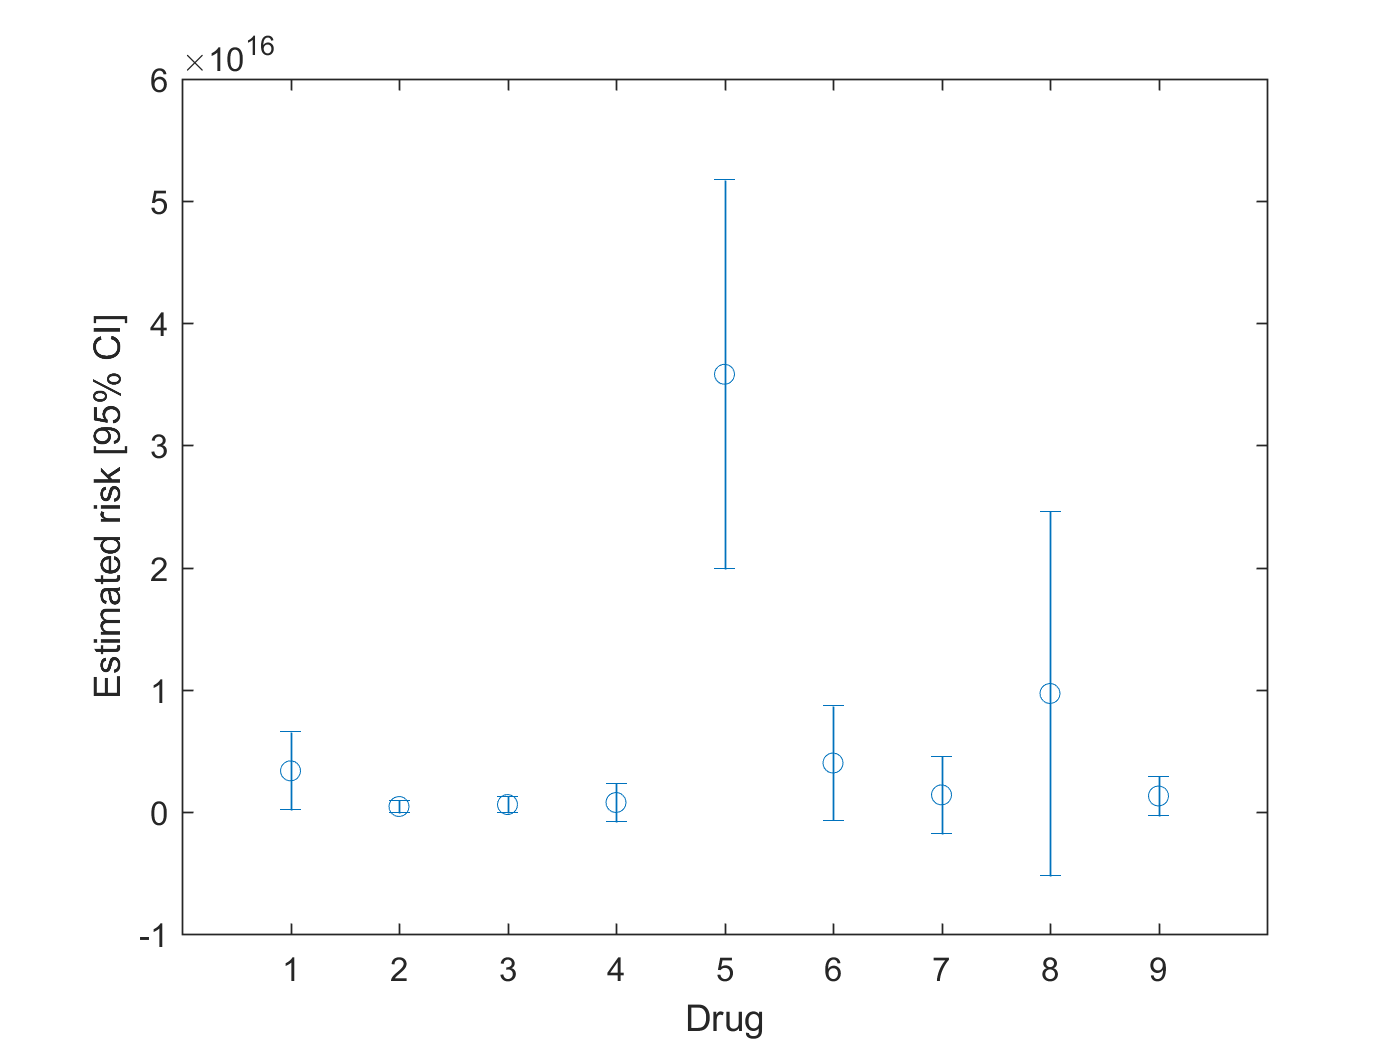
\includegraphics[width = 0.80\textwidth]{Figure/confidense_p1414}
	\caption{Scale values and confidence intervals for the line segments for the second Preference Tree.}
	\label{fig:Tree2conf}
\end{figure}
\noindent
%
When looking at the confidence intervals plotted for the two Preference Trees, it is clear that the second Tree is a better fit. An example is the placement of number five, heroin, clearly different from the other drugs on the confidence plot for the second tree. This is consistent with the plots of the line segments in \autoref{fig:Tree1real} and \autoref{fig:Tree2real} that illustrated that heroin is rated a higher health risk than the other drugs. 